\documentclass[manuscript,screen,review=false, nonacm]{acmart}

\AtBeginDocument{%
  \providecommand\BibTeX{{%
    \normalfont B\kern-0.5em{\scshape i\kern-0.25em b}\kern-0.8em\TeX}}}


\def\@copyrightspace{\relax}
\usepackage{float}
%%\citestyle{acmauthoryear}

\begin{document}

\title[Continual learning vesus robustness]{Do solutions for catastrophic forgetting degrade model robustness to naturalistic corruption and adversarial attacks in binary neural networks?}

\author{Tuan Pham}
\email{tuanph18@uchicago.edu}
\affiliation{%
  \institution{The University of Chicago}
  \city{Chicago}
  \state{Illinois}
  \country{USA}
}

\author{Amit Pradhan}
\email{pradhanak@uchicago.edu}
\affiliation{%
  \institution{The University of Chicago}
  \city{Chicago}
  \state{Illinois}
  \country{USA}
}

\author{Sebastian Barrios}
\email{sebastian.barrios@chicagobooth.edu}
\affiliation{%
  \institution{The University of Chicago}
  \city{Chicago}
  \state{Illinois}
  \country{USA}
}


\keywords{neural networks, catastrophic forgetting, continual learning, robustness, natural corruptions, adversarial attacks}

\maketitle

\section{Introduction}
Developing a deep learning model, for example, in image classification, is not only about achieving the best classification accuracy. Even with increasing computational power, multiple issues also need to be solved, including - to name a few - fast inference time, manageable memory size, continual learning, and robustness to data/model corruption. An attractive solution for fast computation, efficient power consumption, and potentially more straightforward hardware implementation is binary neural networks (BNN) \cite{DBLP:journals/corr/CourbariauxB16}, in which only the signs of the model’s hidden weights are utilized during inference. 

A recent study takes inspiration from biological metaplasticity to solve catastrophic forgetting (CF) problems for continual learning in BNN \cite{Laborieux_Ernoult_Hirtzlin_Querlioz_2021}. More specifically, by creating a form of multiplicative gating during learning for hidden weights to represent weight consolidation (\autoref{fig:fig1}), they are able to solve the permuted-MNIST task, sequential learning with CIFAR-10/100 dataset, and stream learning with these datasets. This approach shares certain similarities with another study in regular neural networks, also inspired by neuroscience literature, which takes into account (a) weight stabilization based on task importance, combined with (b) context-dependent gating allowing for more sparse, non-overlapping population activations, to facilitate learning and remembering a large number of tasks \cite{Masse_2018}. 

Back to BNNs, due to such quantization, they can be quite sensitive to corruption, for example, adversarial data attacks \cite{Lin_2019} or potential soft errors in hardware accelerators \cite{Khoshavi2020}. Hence, we wish to ask whether previous solutions for CF \cite{Laborieux_Ernoult_Hirtzlin_Querlioz_2021} could further degrade model robustness to data corruption or help ameliorate it. 

More specifically, we partially reproduced the results of the metaplasticity training in the permuted MNIST task and the split-class CIFAR task. Then we tested the resulting models under different types of naturalistic corruption to input data are introduced \cite{Hendrycks_2018} and different types of adversarial attacks \cite{rauber2017foolboxnative,rauber2017foolbox,Goodfellow2014-bu}. We also included the Lipschitz regularization term as proposed for defensive quantization \cite{Lin_2019} in the pMNIST task. 

While metaplasticity for BNN was helpful in preventing catastrophic forgetting (pMNIST and split-class CIFAR tasks), the resulting models were not as robust. There appears to be a trade-off for continual learning and robustness, as optimized for the latter would degrade the former, though not in a monotonic manner. Additionally, for the pMNIST task, Lipschitz regularization has mixed effects on model robustness for attacks and corruptions for the pMNIST task.

\section{Methods}

The repository is at \url{https://github.com/tuanpham96/bnn-cf-vs-robust/}

\subsection{Binarized neural networks}

BNN uses binary weights and activations during the inference phase and the training phase binary weights, while the hidden weights are used for training. For the pMNIST task, the BNN is an MLP with 2 hidden layers of varying widths. For the split-class CIFAR, the BNN is a CNN pretrained on ImageNet followed by a metaplastic classifier.

\subsection{Metaplasticity}

The metaplasticity algorithm is shown in \autoref{fig:fig1}d (adapted from \cite{Laborieux_Ernoult_Hirtzlin_Querlioz_2021}), which controls how plastic the hidden weights are. The function $f_{\mathrm{meta}}$ controls how much these weights could be trained - higher hidden weights values indicate more consolidation and disallows further changes. The choice of the function is $1 - \mathrm{tanh}(m \cdot W^h)$ similar to the original paper. The values of the metaplasticity variable $m$ (used interchangeably with \texttt{meta} throughout the text) are varied.  

\begin{figure}[ht]
    \centering
    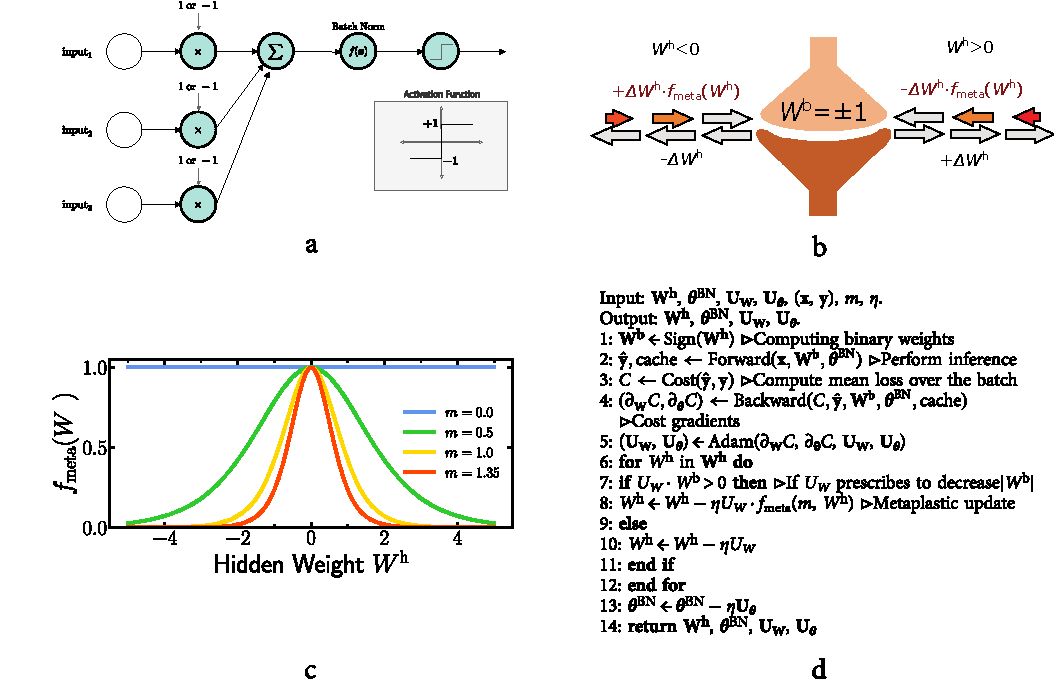
\includegraphics[width=\textwidth]{figures/report/Fig1.pdf}
    \caption{
    Metaplasticity in BNN.
    (\textbf{a}) A typical BNN. 
    (\textbf{b}) Visual representation of metaplasticity (adapted from \cite{Laborieux_Ernoult_Hirtzlin_Querlioz_2021}).
    (\textbf{c}) Plot of hidden weights $W^h$ varying by metaplasticity level $m$ (adapted from \cite{Laborieux_Ernoult_Hirtzlin_Querlioz_2021}).
    (\textbf{d}) Metaplasticity algorithm for BNN (adapted from \cite{Laborieux_Ernoult_Hirtzlin_Querlioz_2021}).
    }
    \label{fig:fig1}
\end{figure}

\subsection{Lipschitz regularization}

This was introduced in \cite{Lin_2019} as an additional regularization term for improving the robustness of quantized networks against adversarial attacks: $\mathcal{L}_{\mathrm{DQ}} = \frac{1}{2}\beta_{\mathrm{DQ}}\sum \lVert \mathbf{W}^T\mathbf{W} - \mathbf{I} \rVert^2$. Briefly, this form of regularization keeps the spectral norm of the hidden weights close to 1 to prevent propagated errors to ``explode''. 

\subsection{Tasks}

The pMNIST task consists of 6 permuted MNIST tasks in which the pixel locations are varied from one task to another. The split-class CIFAR(10/100) task consists of 2 (for CIFAR 10) and 6 (for CIFAR 100) subsets of class. The goal is to achieve high performance in all tasks in an incremental learning scenario without access to previous trained task. 
\subsection{Natural corruption}

The naturalistic corruption transformations are taken from \cite{Hendrycks_2018}. The examples are shown in \autoref{fig:fig2} for the pMNIST task and \autoref{fig:supp1} for the CIFAR task. For the pMNIST dataset, we modified the code te{Hendrycks_2018} to allow for monochrome natural corruptions on. Because some of these transformations are not easily standardized for tensor transformation, these corrupted data sets are pre-generated before training, to save time during testing. Additionally, only one level of severity is tested for all of natural corruptions.

\begin{figure}[ht]
    \centering
    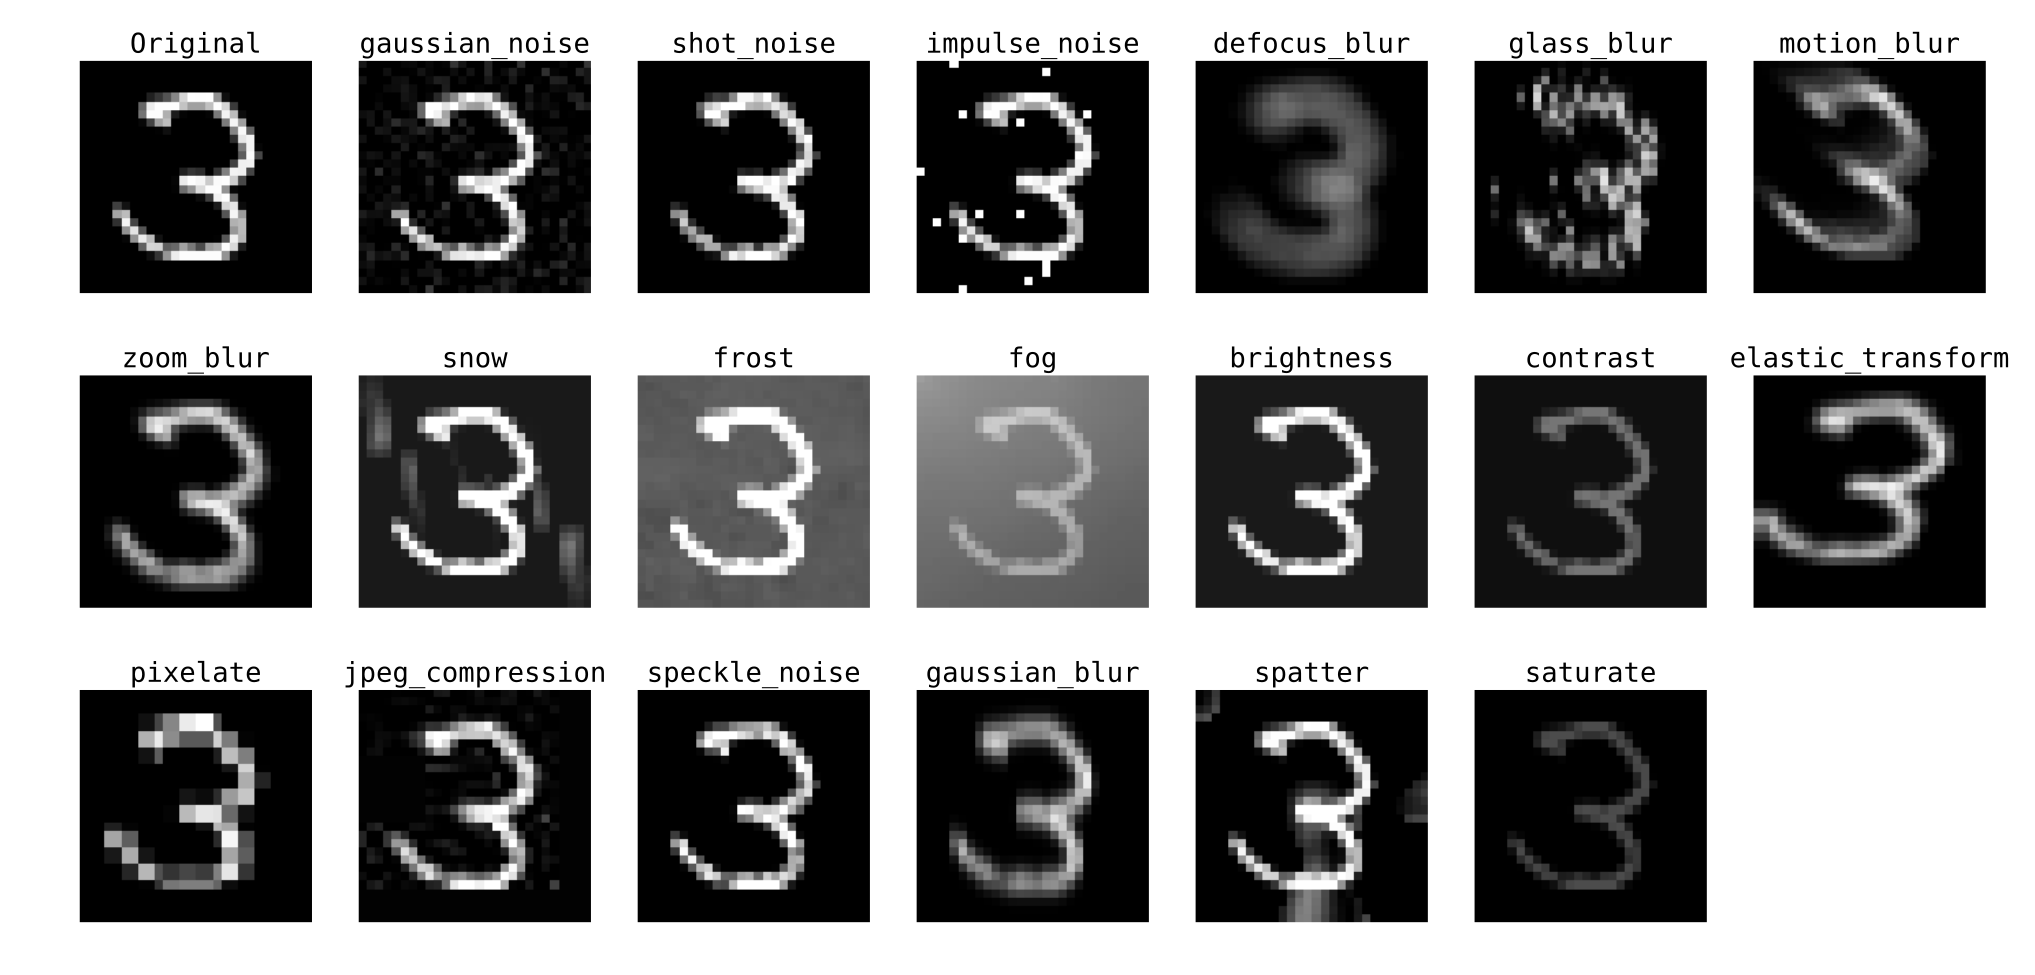
\includegraphics[width=\textwidth]{figures/report/Fig2.png}
    \caption{Natural corruption applied to the MNIST dataset.}
    \label{fig:fig2}
\end{figure}

\subsection{Adversarial attacks}

The adversarial attacks are small perturbations (with varying magnitudes $\epsilon$) applied to these tasks are targeted attacks, taken from \cite{rauber2017foolbox,rauber2017foolboxnative}. Due to the limited time, we were not able to integrate the various attacks to the CIFAR task (only self-coded FGSM). Briefly, the attacks covered here are:

\begin{itemize}
    \item \texttt{Additive-Uniform-Noise} is not a targeted attack, with only small addtive noise sampled a from uniform distribution. This serves as a reference as this would suffer less damage than the following targeted attacks. 
    \item \texttt{FGSM} (Fast Gradient Sign Method) \cite{Goodfellow2014-bu} is a white-box attack that applies small perturbations following the sign of the loss gradients for the current input. 
    \item \texttt{Basic-Iterative-Attack} \cite{Kurakin2016-mb} and \texttt{PGD} (Projected Gradient Descent) \cite{Madry2017-dx} are \texttt{FGSM} extensions that allow for iterative \texttt{FGSM} perturbations with magnitude clipping. The latter starts with additive signs of a sampled Gaussian distribution, in addition to \texttt{FGSM}.
    \item \texttt{DeepFool-Attack} \cite{Moosavi-Dezfooli2016-qf}  approximates the model linearly and iteratively chooses the pertubation to cross model decision boundary. 
    \item \texttt{DDN-Attack} (Decoupled Direction and Norm)  \cite{Rony2018-tp} projects the perturbation directions onto an $\epsilon$ sphere and further adjusts the sphere radius depending on whether the generated input is considered adversarial. 
\end{itemize}

For the pMNIST adversarial evaluation, instead of looking at the monotonically decreasing accuracy-perturbation curves directly, we calculated the normalized area under the curve (\texttt{auc\_log}) of the log-log plot with controled for the minimum accuracy ($a_{\mathrm{min}} = 1e-4$ instead of 0.0) and minimum $\epsilon_{\mathrm{min}}$ (0.9 of the second smallest $\epsilon$ instead of 0.0). In other words: $ \texttt{auc\_log} = \mathrm{trapz}(\log a - \log a_{\mathrm{min}} ,\log \epsilon - \log \epsilon_{\mathrm{min}}) / |\log a_{\mathrm{min}} \times \log  \epsilon_{\mathrm{min}}| $

\section{Results}

\subsection{Permuted MNIST task}

\subsubsection{Replication of BNN training with metaplasticity parameter for the pMNIST task}

\begin{figure}[ht]
    \centering
    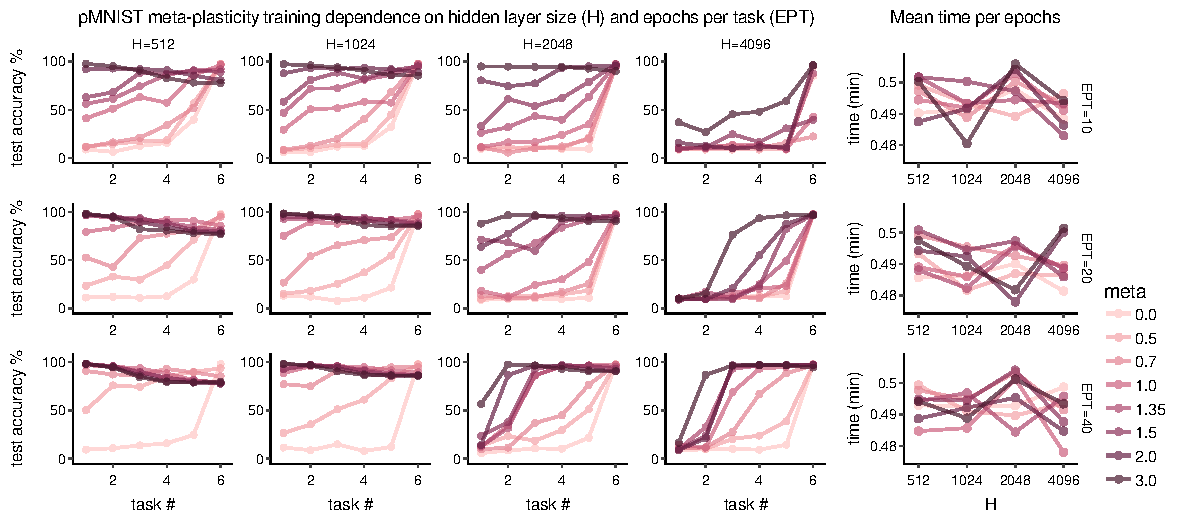
\includegraphics[width=1.1\textwidth]{figures/report/Fig3.pdf}
    \caption{
    Results of permuted MNIST tasks for the BNNs with metaplasticity training for different variations of \texttt{meta} (colors), network widths $H$ (left to right), number of epochs per task (EPT, top to bottom). The leftmost column shows the average time taken to train the model. 
    }
    \label{fig:fig3}
\end{figure}

Before applying corruptions to the dataset, we first set out to observe whether the original results from \cite{Laborieux_Ernoult_Hirtzlin_Querlioz_2021} were replicable. So we ran their codes for the multipercepton (MLP) version of the BNN with 2 hidden layers for different values of the \texttt{meta} hyperparameters: low \texttt{meta} means binary hidden weights are allowed to change easily while high means such weights’ own plasticity is constrained by their magnitude. In addition, we also varied the widths of the hidden layers ($H$) and the number of training epochs per task (EPT), for a total of only 6 tasks. This is shown in \autoref{fig:fig3}). 

Consistent with the paper, higher \texttt{meta} leads to better performance (potentially criticality is around 1.0), in which earlier tasks still perform well. Interestingly, too high \texttt{meta} could lead to some degradation (though still good) for more recent tasks - this is possibly because high values would bias most changes happening for earlier tasks and consolidate many hidden weights from early ones. Regardless, these results confirm the benefits of the metaplasticity to solve the pMNIST task, which is one of the benchmarks for catastrophic forgetting. Surprisingly, the average time taken to train each epoch did not vary significantly between different types of variations shown here  

However, contrary to the benefits from increased hidden layer widths shown in the original paper, we found that large networks could be harmful. The peak performance is around $H=1024$ but further model width increase decreases performance even in comparison to the $H=512$ network tested here. We hypothesized that maybe larger networks would require more time to balance consolidation and learning. Hence we varied EPT (in the paper EPT=40), but we never could replicate the size effects, for multiple runs on multiple different machine resources. Currently, we do not have any explanation for this. 

\subsubsection{Lipschitz regularization}

\begin{figure}[ht]
    \centering
    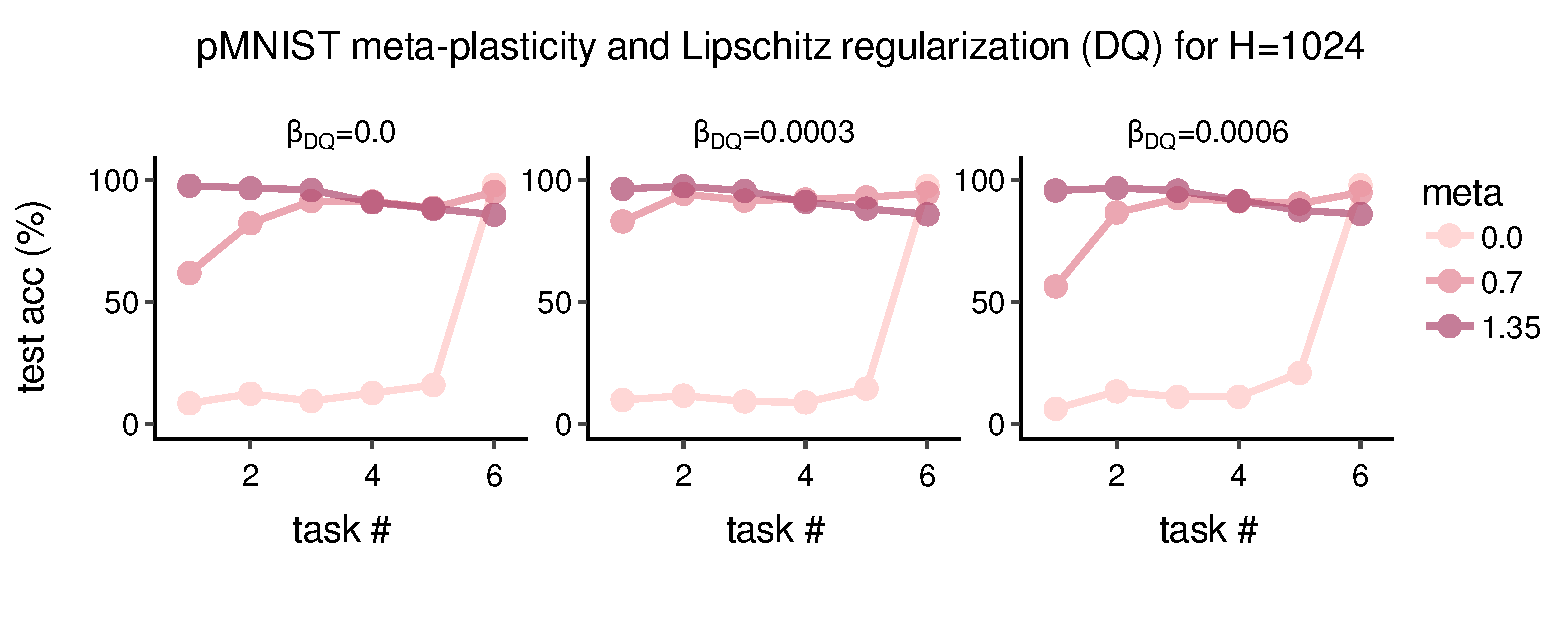
\includegraphics[width=0.65\textwidth]{figures/report/Fig4.pdf}
    \caption{The effects of Lipschitz regularization importance $\beta_{\mathrm{DQ}}$ (left to right) to the pMNIST task in addition to the metaplasticity training (colors)}
    \label{fig:fig4}
\end{figure}

In addition, we also tested the Lipschitz regularization for improving the robustness of quantized neural networks \cite{Lin_2019} on top of metaplasticity training. We chose the hyperparameter $\beta_{\mathrm{DQ}}$ similar to the original paper on defensive quantization (DQ). Intriguingly, these two processes counteract each other to some extent in \autoref{fig:fig4}, as the medium value of $\beta_{\mathrm{DQ}}$ improves slightly catastrophic forgetting, but the largest value here degrades it, especially for medium \texttt{meta} hyperparameter. 

However, one drawback of the metaplasticity method not explicitly mentioned in the main text is the reliance on task-relevant batchnorm states. According to the authors \cite{Laborieux_Ernoult_Hirtzlin_Querlioz_2021}, technically, these states are cheap to store relative to weights, but realistically it is not explicitly clear how to load these weights automatically and effectively. Hence, moving forward with perturbation robustness testing for the pMNIST task, we removed this dependence to fairly assess the robust continual learning. 

\subsubsection{Natural corruptions to pMNIST tasks}

\begin{figure}[ht]
    \centering
    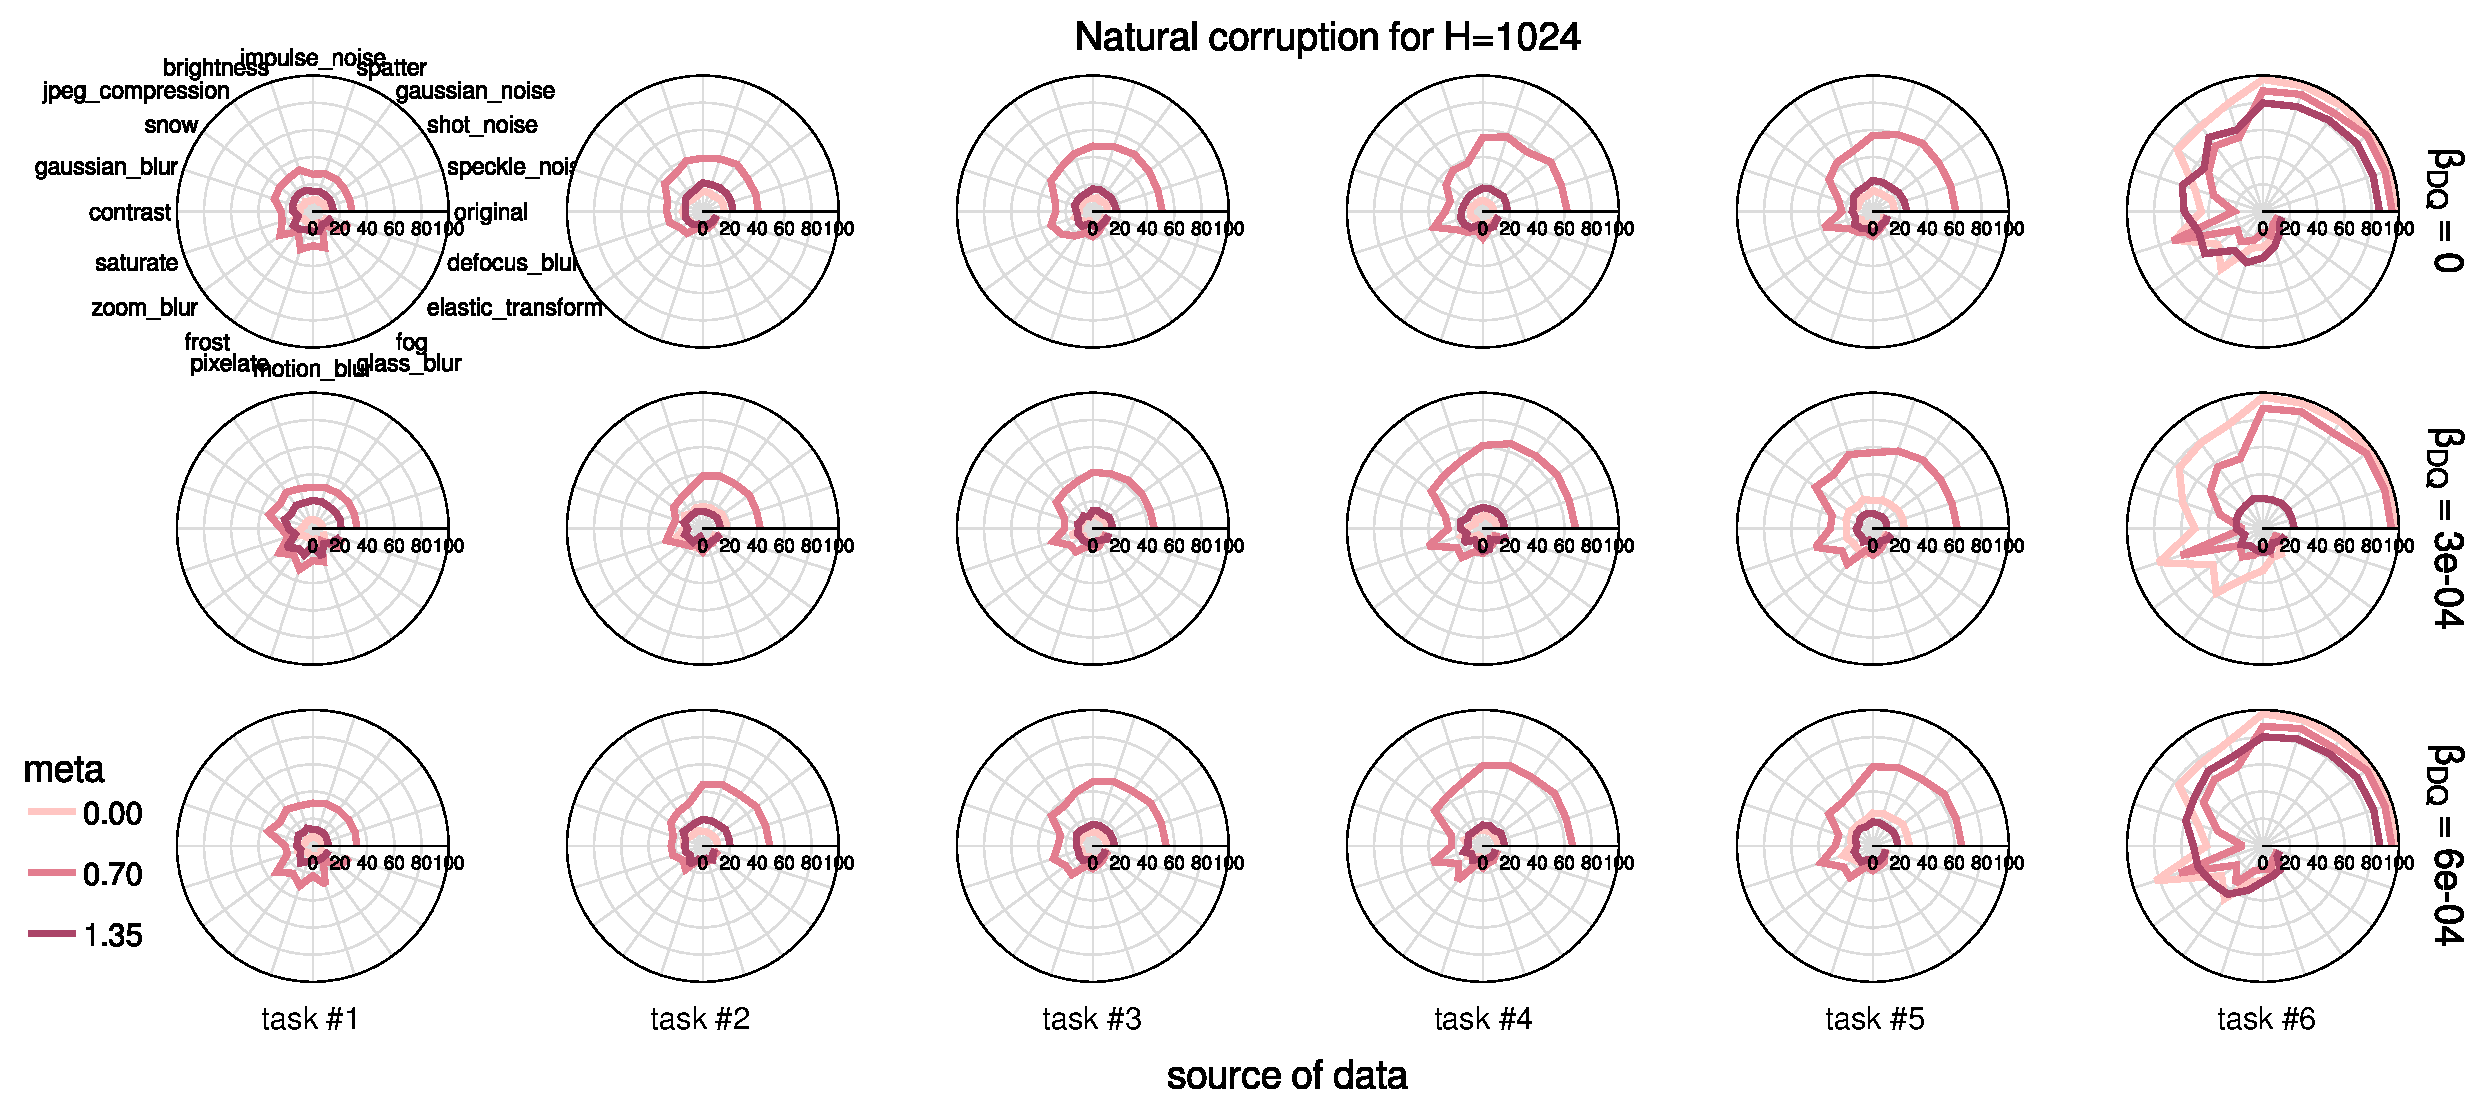
\includegraphics[width=1.1\textwidth]{figures/report/Fig5.pdf}
    \caption{
    Natural corruption robustness after metaplasticity training (colors) and Lipschitz regularization (top to bottom) in the pMNIST task. 
    From left to right is the source of the task data. 
    The radius shows the test accuracy due to these different perturbation methods (different angles, with the original at $0^{\circ}$).
    }
    \label{fig:fig5}
\end{figure}

Next, we moved on to applying perturbations onto our MNIST and pMNIST datasets after training the BNN models with metaplasticity optimization and Lipschitz regularization. The examples of these corruption transformations are shown in \autoref{fig:fig2}. It must be noted that these types of corruption are possibly more realistic when considered with colored images like CIFAR or ImageNet, and the more appropriate benchmarks for catastrophic forgetting coupled with these types of perturbations would be MNIST-FMNIST or split-class CIFAR. Regardless, for now, we chose permuted MNIST as our first approach to assess catastrophic forgetting with natural corruptions.

The results are shown in \autoref{fig:fig5} for the models at the end of training for different values of \texttt{meta}. First, note that removing the task-relevant batchnorm states here reveals the model's accuracy for the original case, though the metaplasticity training preserves some nontrivial performance but not qualified for continual training. However, although the effect of magnitude is debatable, the inclusion of metaplasticity improves robustness against many other naturalistic corruptions, but, as expected, not so much for the most current task. The inclusion of the Lipschitz regularization has quite mixed effects, as there appears to be both cases of improvements and degradations for earlier tasks. 

\subsubsection{Adversarial attacks to pMNIST tasks}

\begin{figure}[ht]
    \centering
    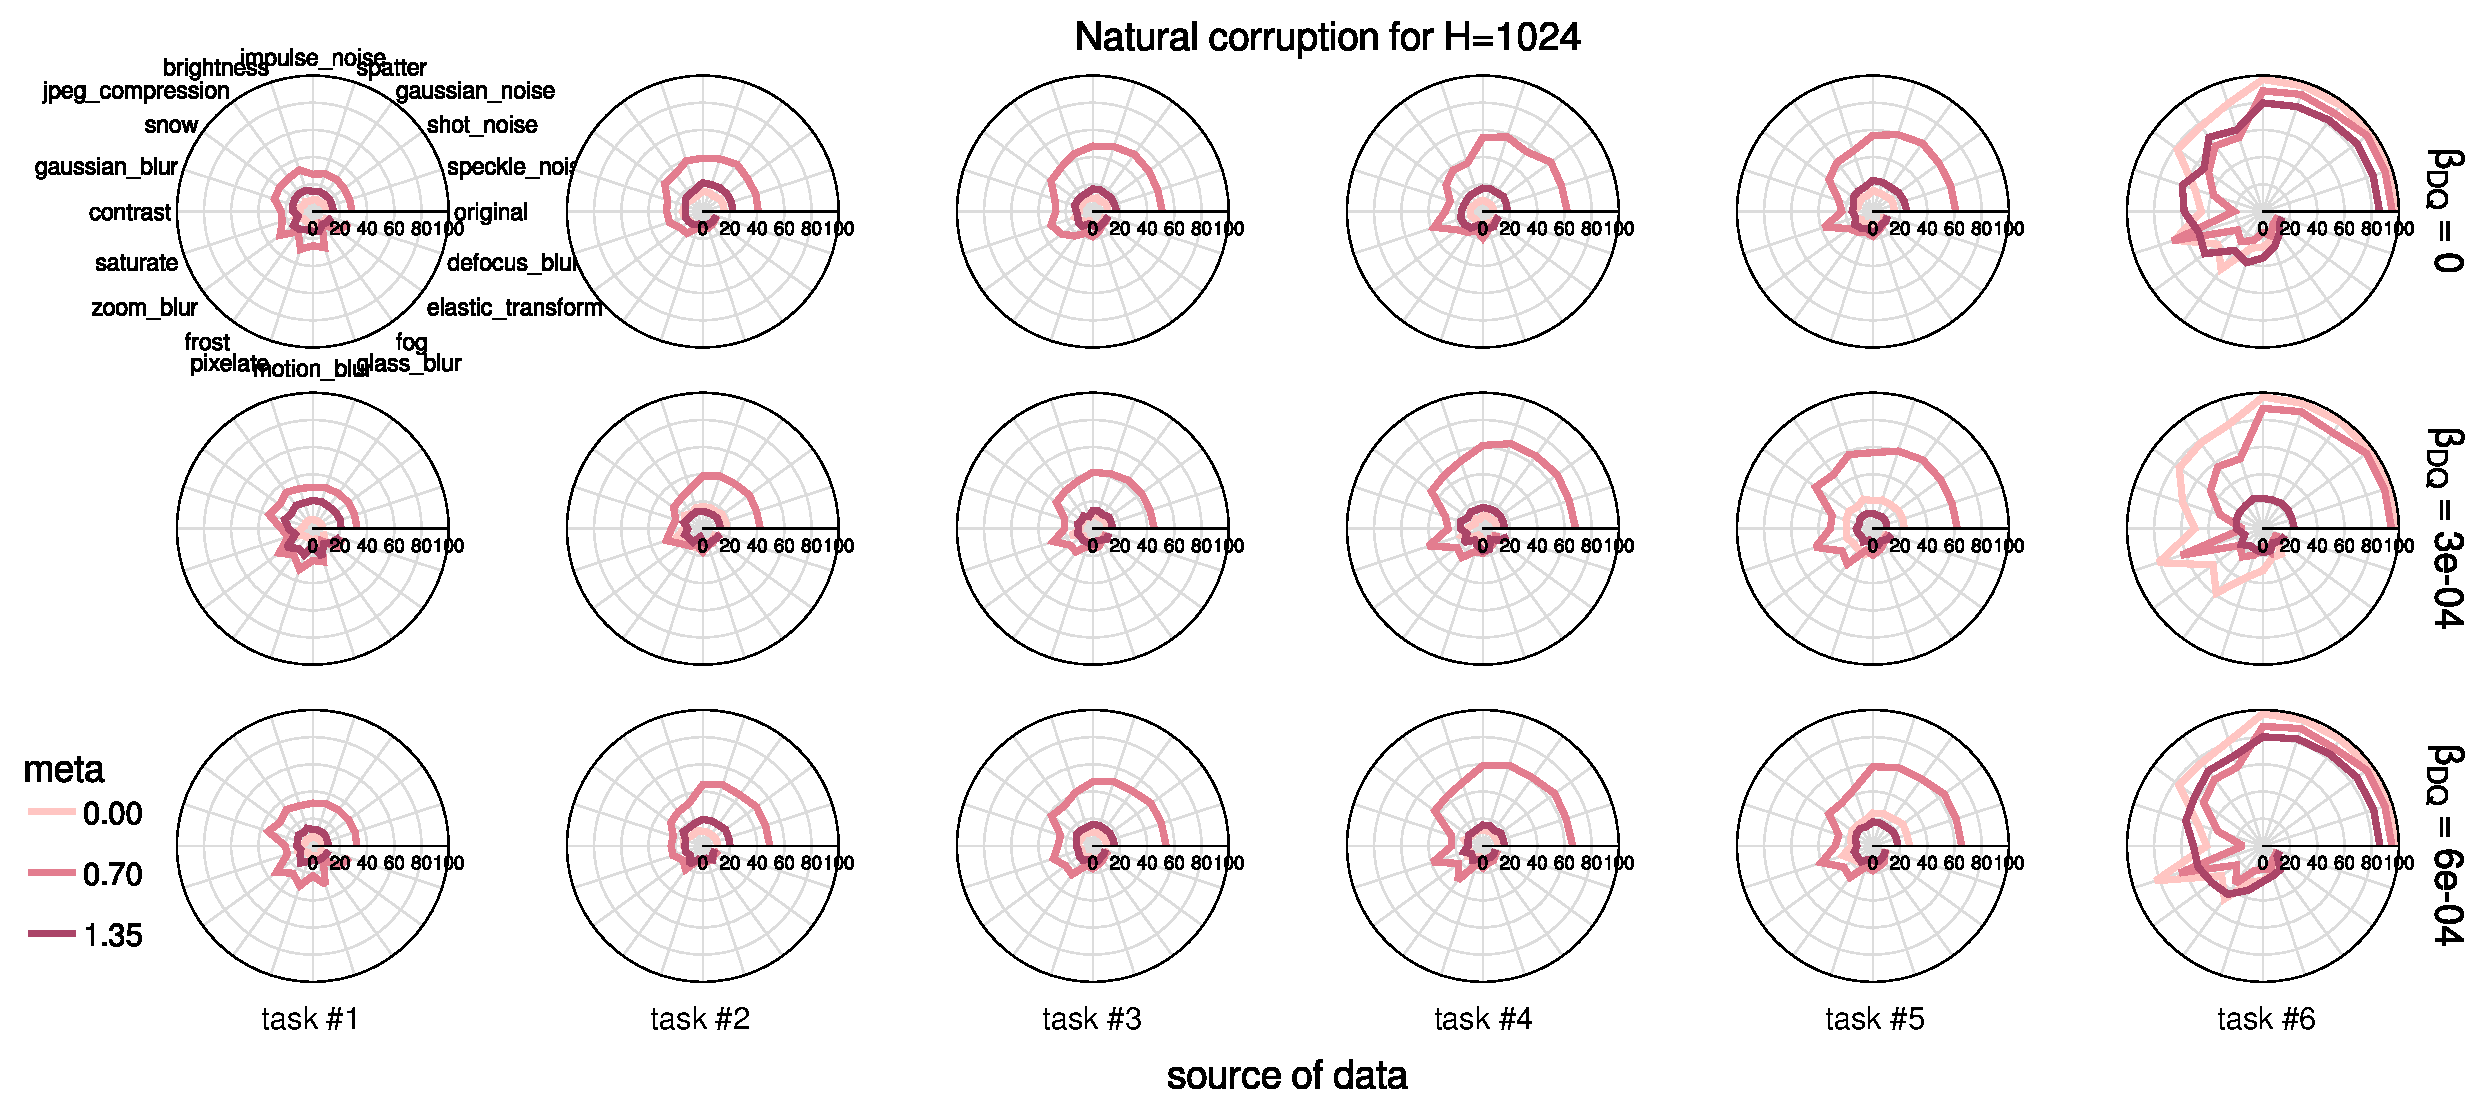
\includegraphics[width=1.1\textwidth]{figures/report/Fig6.pdf}
    \caption{
    Adversarial robustness after metaplasticity training (colors) and Lipschitz regularization (top to bottom) in the pMNIST task. From left to right is the source of the task data. 
    The radius shows the calculated log (to see the difference) of \texttt{auc\_log} due to these different perturbation methods (different angles, with the original at $0^{\circ}$). 
    See methods for more information on the types of adversarial attacks and the calculation of \texttt{auc\_log}.
    }
    \label{fig:fig6}
\end{figure}

Lastly, for the pMNIST task, we used different adversarial attacks and calculated the \texttt{auc\_log} as a way to assess the model adversarial robustness after metaplasticity and Lipschitz regularization (see Methods). The results are shown in \autoref{fig:fig6}. First, in retrospect, this might not be the most effective way to address adversarial robustness, for example, inspecting a specific range of perturbation rather than considering the whole range would have been a better choice. Regardless, the preliminary results shown in \autoref{fig:fig6} reveals the mixed effects of these two processes again. However, for the baseline case without metaplasticity training, the inclusion of this $\beta_{\mathrm{DQ}}$ in the most current task (leftmost column, lightest color) unfortunately does not achieve noticeable benefits. For previous tasks, the inclusion the medium \texttt{meta} hyperparameter seems to improve robustness but the effect of $\beta_{\mathrm{DQ}}$ again does not seem clear. Future experiments should take into account adversarial training in addition to the Lipschitz regularization as suggested in the original paper \cite{Lin_2019}.

\subsection{Class Incremental Learning on CIFAR-100 Features}

\begin{figure}[ht]
    \centering
    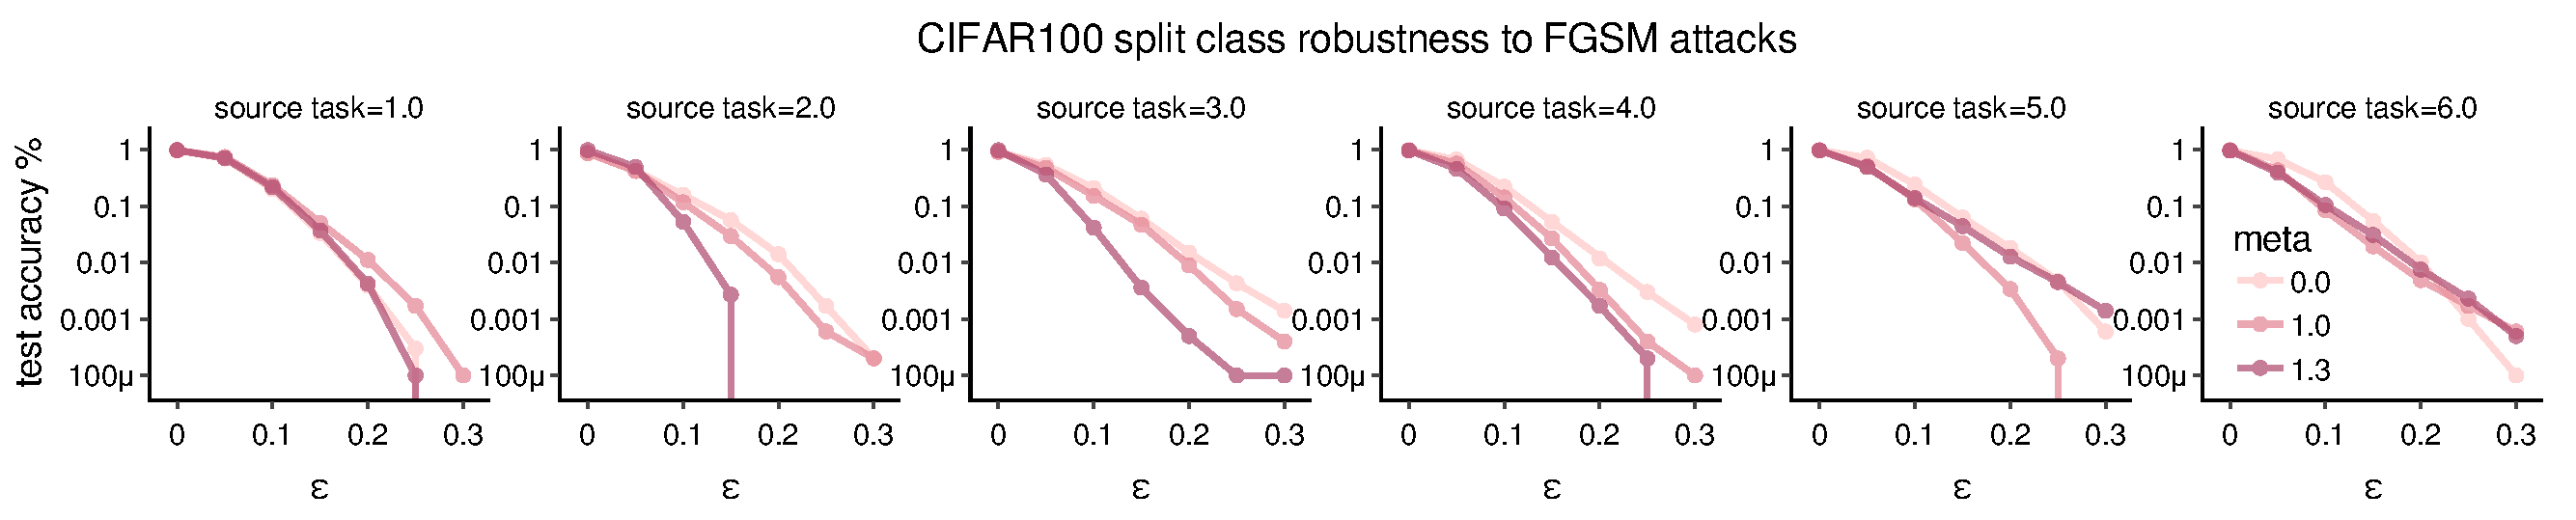
\includegraphics[width=0.8\textwidth]{figures/report/Fig7.pdf}
    \caption{
    Metplasticity training with the class incremental learning on CIFAR datasets. 
    }
    \label{fig:fig7}
\end{figure}

We next experimented with an incremental learning setting where the model learns different subsets of classes of CIFAR-10 and CIFAR-100 datasets. CIFAR-10 was divided into two subsets (animal subset and vehicle subset). Since CIFAR-100 consists of more classes (100 classes), we prepared six subsets based on the class labels. We use a BNN composed of one hidden layer with 2048 neurons for CIFAR-10 and BNN composed of two hidden layers with 2048 neurons each. For the experiment we selected three \texttt{meta} values: 0.0, 1.0, and 1.3; for both of the tasks. The key idea behind these tasks is that learning features from images does not change over time.


\begin{figure}[ht]
    \centering
    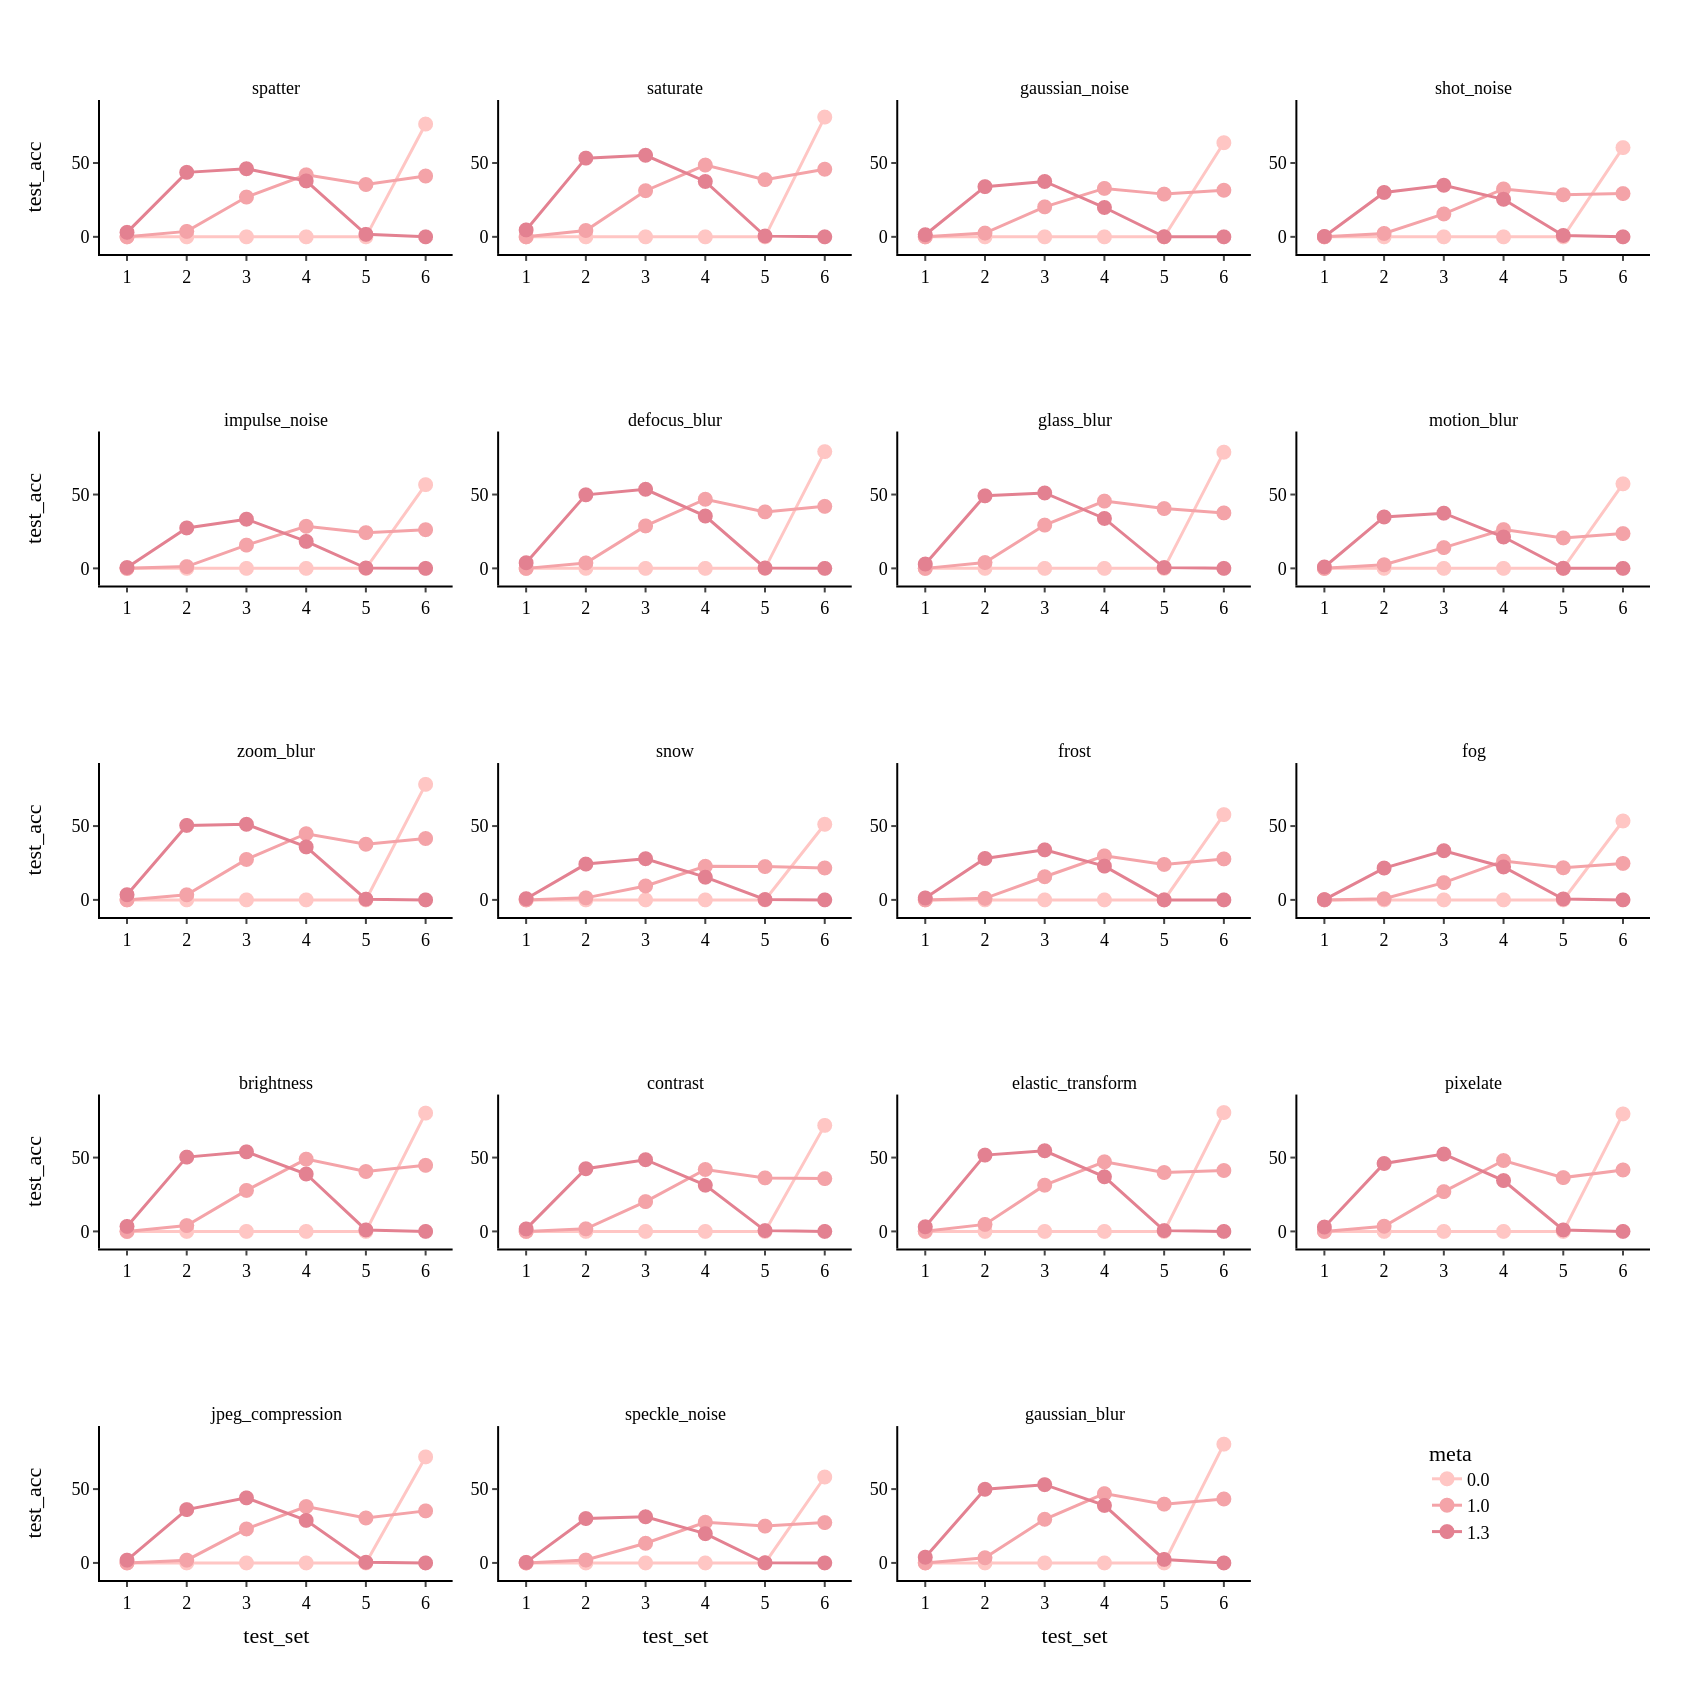
\includegraphics[width=1\textwidth]{figures/report/Fig8.png}
    \caption{Effects of applying various natural corruptions to model accuracy in case of CIFAR-100 dataset, across different \texttt{meta} parameter
    }
    \label{fig:fig8}
\end{figure}

To extract features from CIFAR-10 and CIFAR-100 datasets, we used the convolutional layers of the ResNet-18 network (removing the last layer), which is pretrained on the ImageNet dataset. CIFAR-10 and CIFAR-100 images were reshaped from 32 x 32 pixels to 220 x 220 pixels, randomly cropped using 200 x 200 windows, and randomly flipped (along the vertical axis). We made ten passes through the training dataset to extract 500,000 image features, but only performed one pass through the test dataset to extract 10,000 images. The extracted features were then trained using binarized neural networks, with shapes 512 x 2048 x 10 and 512 x 2048 x 2048 x 100 for CIFAR-10 and CIFAR-100, respectively. 

The results for metaplasticity training with CIFAR datasets are shown in \autoref{fig:fig7}. As expected, without synaptic metaplasticity in the CIFAR-10 dataset, the model ``forgot'' task 1 after learning task 2. Similarly, only the current subset was ``remembered'' for the CIFAR-100 task. For the CIFAR-10 case, $\texttt{meta} = 1.3$ performed the best, but $\texttt{meta} = 1.0$ for CIFAR-100, giving reasonable accuracy values for the last four tasks. One strange observation arose in the case when $\texttt{meta} = 1.3$ for the latter case, the model could not learn the last two tasks at all. We hypothesize that, since a larger \texttt{meta} value makes the model more rigid to changes in the binary weights, tasks 5 and 6 could not be learned. This was qualitatively similar to why high \texttt{meta} values decrease performance slightly as a function of task sequence in \autoref{fig:fig3}.

\subsubsection{Natural corruption to CIFAR split-class task}

We then applied various types of natural corruption to CIFAR-10 and CIFAR-100 datasets, a more realistic approach as natural corruption is most common in the case of colored images. From \autoref{fig:supp2} we can observe that the model accuracy is less affected by the various natural corruptions to CIFAR-10 images. Similar behavior is also observed in \autoref{fig:fig8} for the CIFAR-100 dataset. One possible explanation is that the image features remain intact even after adding a small amount of noise. In fact, we introduced noise into the images in the data preparation step as we scaled up the number of pixels from 32 x 32 to 220 x 220, randomly cropped using a 200 x 200 window, and finally applied random horizontal flips. 

\subsubsection{Adversarial attacks on CIFAR}

We finally tested the performance of BNNs with synaptic metaplasticity models under FGSM attacks (\autoref{fig:fig9}). We can observe the model accuracy rapidly degraded as we increased the amount of epsilon (noise). Synaptic metaplasticity does not seem to provide any resistance to FGSM attack. Unfortunately, we did not have time to test a wide range of adversarial attacks except for the FGSM method for the CIFAR dataset.


\begin{figure}[ht]
    \centering
    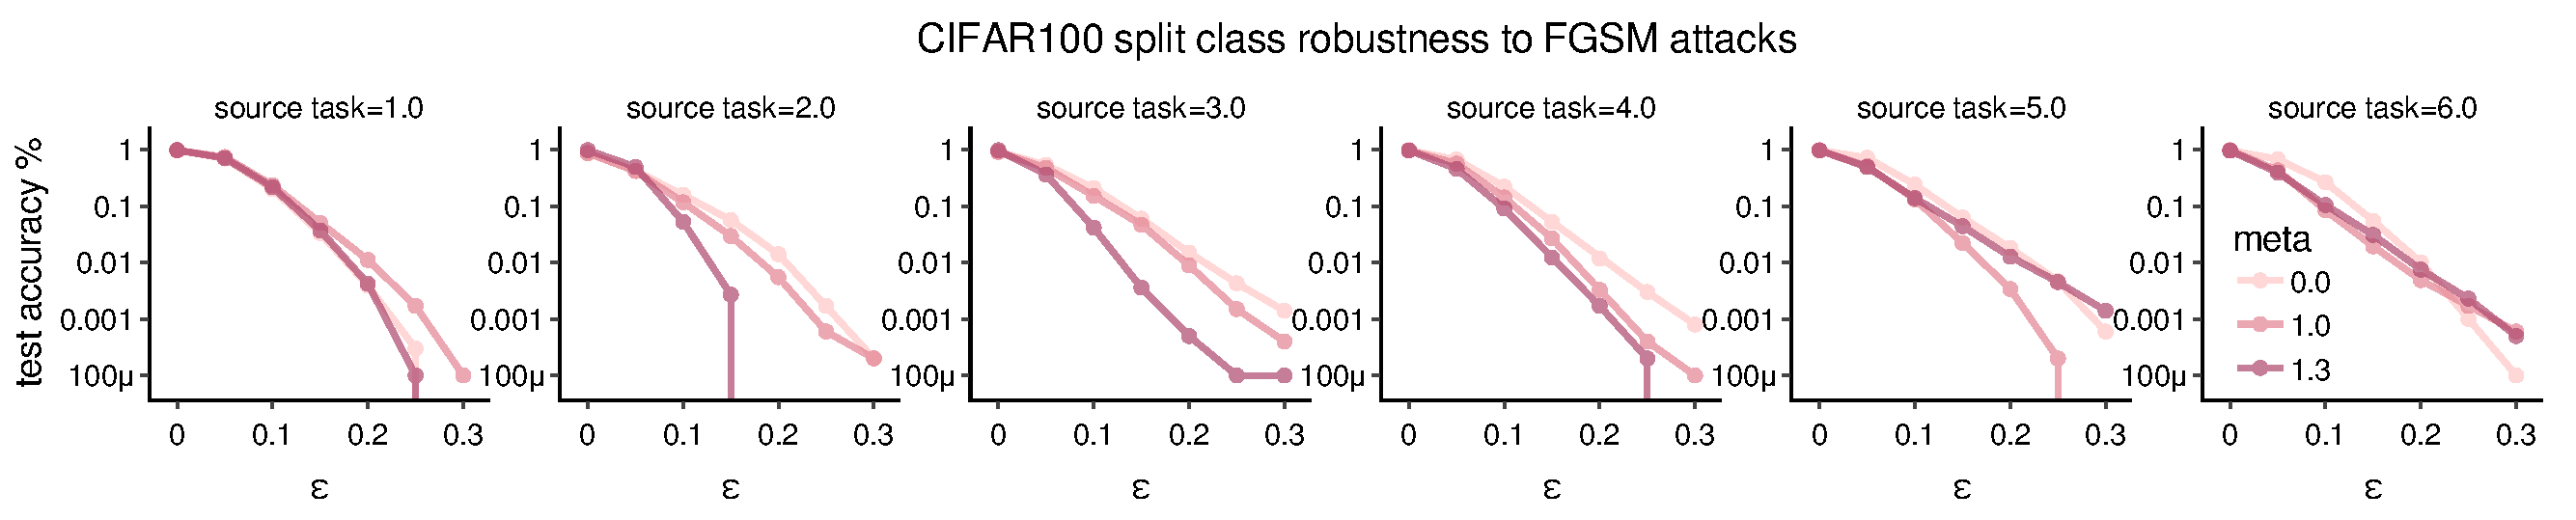
\includegraphics[width=1.1\textwidth]{figures/report/Fig9.pdf}
    \caption{
    FGSM adversarial attack on CIFAR-100 data of the BNN trained with metaplasticity (colors) across the different subsets (left to right), showing the test accuracy as a function of perturbation strengths $\epsilon$.
    }
    \label{fig:fig9}
\end{figure}

\section{Conclusion}

While metaplasticity for BNN helped prevent catastrophic forgetting (pMNIST and split-class CIFAR tasks), the results were not robust. There appears to be a trade-off for continual learning and robustness - only medium values of \texttt{meta} would result in more robust models. Additionally, for the pMNIST task, Lipschitz regularization has mixed effects on model robustness for attacks and corruptions for the pMNIST task.
    
However, there were also issues within the metaplasticity training: (1) dependence on the task-relevant batchnorm states, (2) irreproducible network size benefits as seen in the paper \cite{Laborieux_Ernoult_Hirtzlin_Querlioz_2021}. Plus, we did not have time to assess model compression benefits and speed in comparison with real-valued networks - one reason was that metaplasticity was not effective in such networks. Hence, future experiments should involve 

\begin{enumerate}
    \item more continual learning tasks (e.g., stream learning, MNIST-FMNIST) \cite{Farquhar2018-zz,Van_de_Ven2019-xl,Laborieux_Ernoult_Hirtzlin_Querlioz_2021}
    \item more systematic comparisons (performance, time, inference, memory cost, robustness) between different known solutions for catastrophic forgetting (e.g. elastic weight consolidation \cite{Kirkpatrick2017-pe}, contextual gating \cite{Masse2018-ms}, synaptic intelligence \cite{Zenke2017-zl}) for neural networks across different quantization levels, as well as the continuous-valued networks
    \item combination of robustness improvement training including revisiting Lipschitz regularization \cite{Lin_2019}, data augmentation for natural corruptions and adversarial training \cite{Madry2017-dx}. 
\end{enumerate}

\bibliographystyle{ACM-Reference-Format}
\bibliography{bibliography}

\setcounter{figure}{0}
\renewcommand{\thefigure}{S\arabic{figure}}

\section{Supplemental Figures}
\begin{figure}[ht]
    \centering
    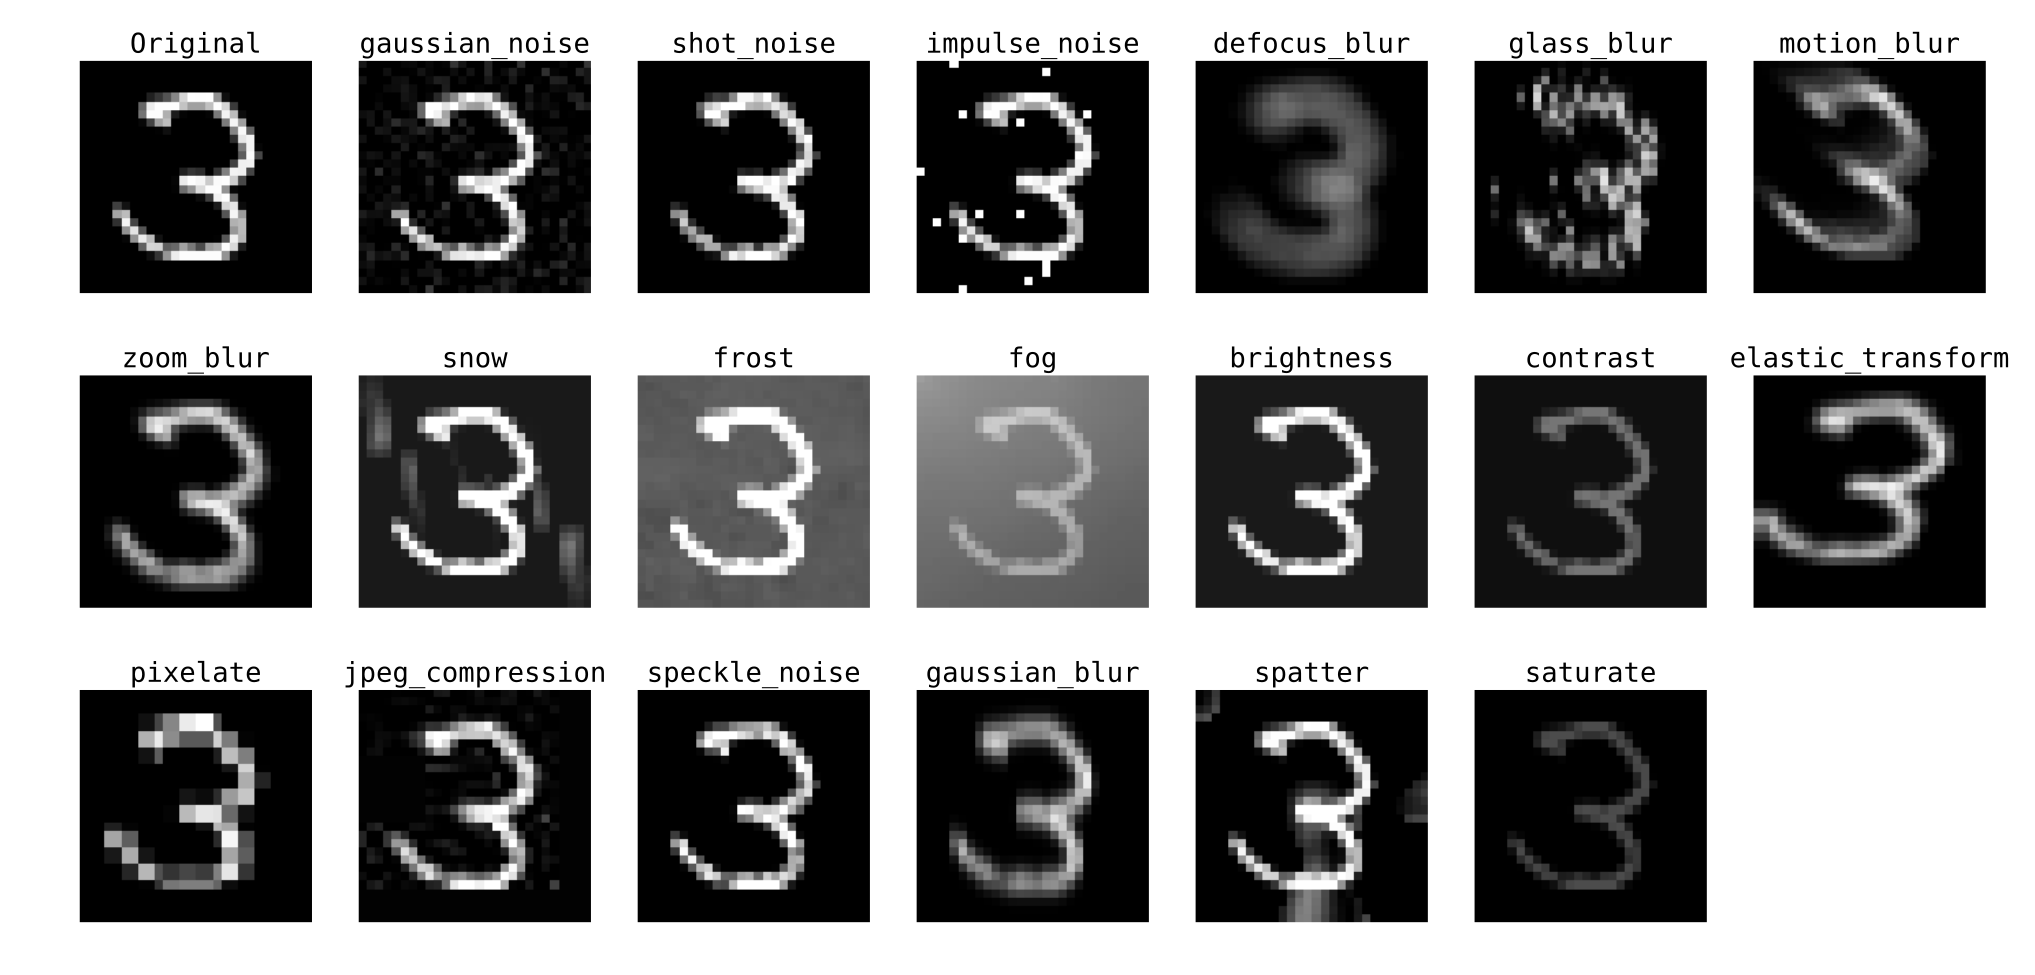
\includegraphics[width=1.1\textwidth]{figures/report/FigS1.png}
    \caption{Natural corruption applied to the CIFAR dataset.}
    \label{fig:supp1}
\end{figure}


\begin{figure}[ht]
    \centering
    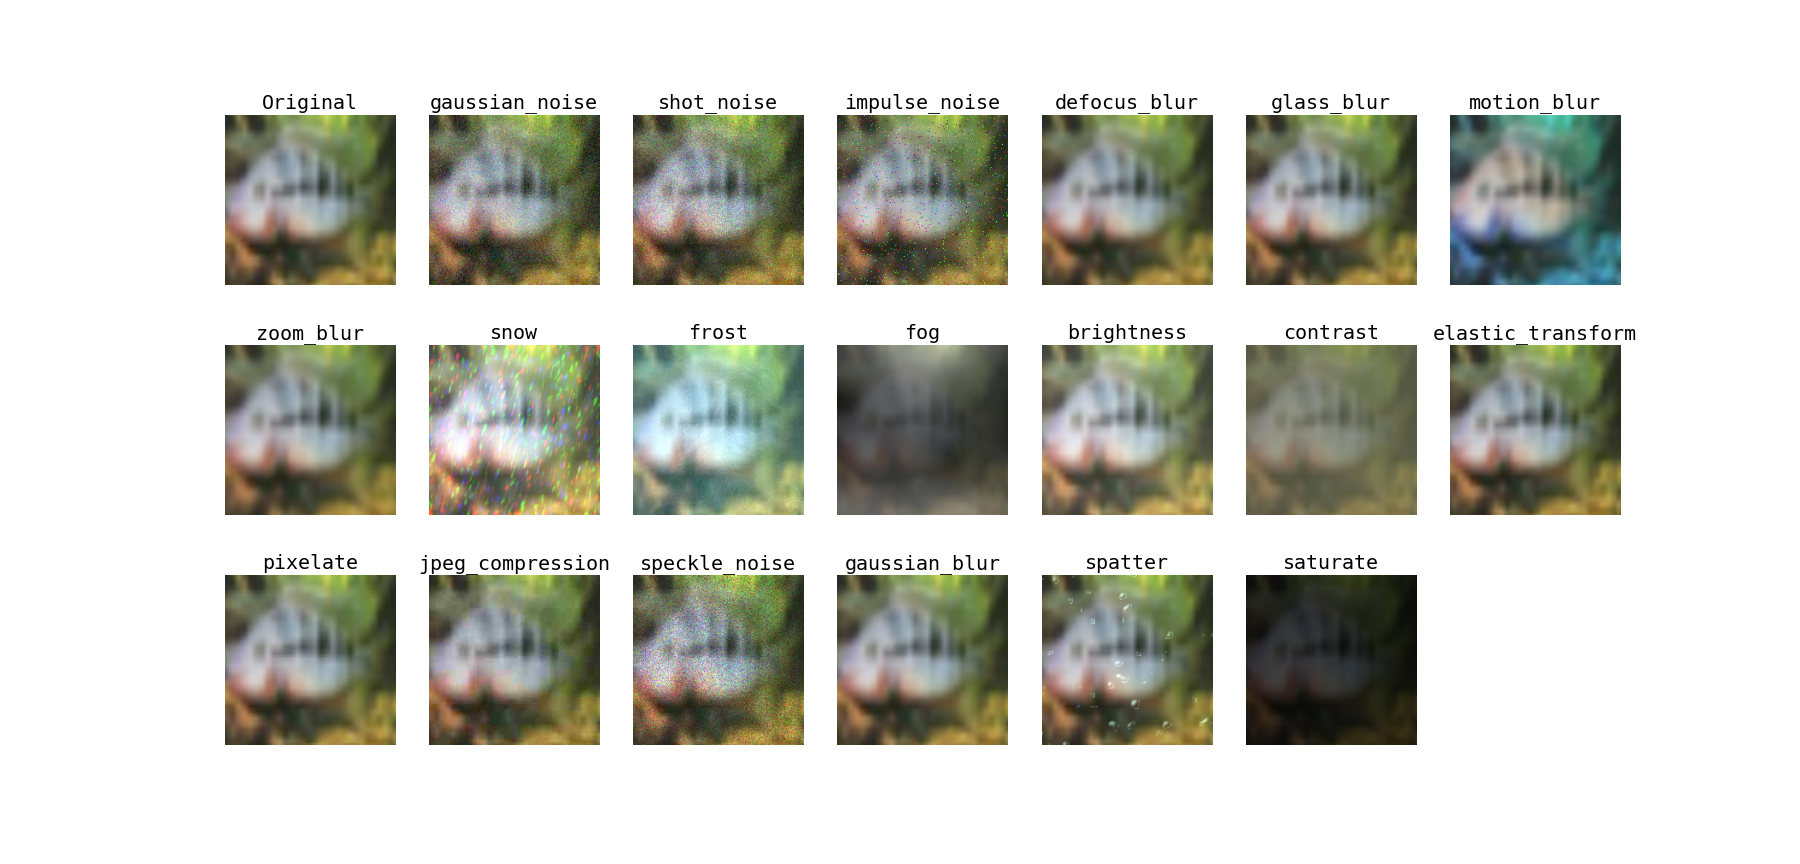
\includegraphics[width=1.1\textwidth]{figures/report/FigS2.png}
    \caption{Effects of applying various natural corruptions to model accuracy in the case of the CIFAR-10 dataset.}
    \label{fig:supp2}
\end{figure}

\end{document}
\endinput
